% Preamble {{{
\documentclass[]{beamer}
\usepackage{ngerman}

\providecommand\thispdfpagelabel[1]{}

\usepackage[utf8]{inputenc}
%\usepackage[T1]{fontenc}
\usepackage{cite}

\usepackage{verbatim}

\usepackage{amssymb}

\usepackage{graphics}

\usepackage{tikz}
\usetikzlibrary{shapes,fadings}

\usepackage{hyperref}

\tikzstyle{blob}=[rectangle,
	thick,
	minimum size=0.8cm,
	draw=purple!80,
	fill=purple!20]

\tikzstyle{tree}=[rectangle,
	thick,
	minimum size=0.8cm,
	draw=blue!80,
	fill=blue!20]

\tikzstyle{commit}=[rectangle,
	thick,
	minimum size=0.8cm,
	draw=green!80,
	fill=green!20]

\tikzstyle{branch}=[rectangle,
	thick,
	minimum size=0.8cm,
	draw=yellow!80,
	fill=yellow!20]

\tikzstyle{tag}=[rectangle,
	thick,
	minimum size=0.8cm,
	draw=orange!80,
	fill=orange!20]

% Preamble }}}
%\definecolor{OneFg}{RGB}{0,0,0}
%\definecolor{OneBg}{RGB}{161,255,135}
%\definecolor{TwoFg}{RGB}{0,0,0}
%\definecolor{TwoBg}{RGB}{9,249,198}
%\definecolor{ThreeFg}{RGB}{0,0,0}
%\definecolor{ThreeBg}{RGB}{255,107,33}
%\definecolor{FourFg}{RGB}{255,255,255}
%\definecolor{FourBg}{RGB}{239,163,122}
%\definecolor{FiveFg}{RGB}{0,0,0}
%\definecolor{FiveBg}{RGB}{177,229,237}

\definecolor{OneFg}{RGB}{0,0,0}
\definecolor{OneBg}{RGB}{209,242,165}
\definecolor{TwoFg}{RGB}{0,0,0}
\definecolor{TwoBg}{RGB}{239,250,180}
\definecolor{ThreeFg}{RGB}{0,0,0}
\definecolor{ThreeBg}{RGB}{255,196,140}
\definecolor{FourFg}{RGB}{0,0,0}
\definecolor{FourBg}{RGB}{255,159,128}
\definecolor{FiveFg}{RGB}{0,0,0}
\definecolor{FiveBg}{RGB}{245,105,145}

\definecolor{FooFg}{RGB}{84,36,55}
\definecolor{FooBg}{RGB}{250,211,178}

\definecolor{Christian}{RGB}{0,102,204}

% \usebackgroundtemplate{
% 	\includegraphics[width=\paperwidth, height=\paperheight]{foo.pdf}
% }
\newcommand{\normalstyle}{
	\setbeamercolor{background canvas}{bg=}
	\setbeamercolor{frametitle}{fg=FooFg}
}

\newcommand{\styleFoo}{
	\setbeamercolor{background canvas}{bg=FooBg}
	\setbeamercolor{frametitle}{fg=FooFg}
}

\newcommand{\styleOne}{
	\setbeamercolor{background canvas}{bg=OneBg}
	\setbeamercolor{frametitle}{fg=OneFg}
}

\subject{Version Control -- eine Einführun}

\newcommand{\todo}{\textcolor{red}{\textbf{ \textsf{TODO} }}\\}


\begin{document}
\setbeamercolor{frametitle}{fg=Christian}
\setbeamercolor{framesubtitle}{fg=Christian}
\setbeamercolor{item}{fg=Christian}

\title[Version Control]{Version Control -- eine Einführung}
\subtitle[Zoran Zari\'c]{Zoran Zari\'c}
\author[Zoran Zari\'c]{Zoran Zari\'c}

\begin{frame}
	\fontsize{30}{10}\selectfont Version Control
	\vspace*{0.5cm}

	\fontsize{20}{10}\selectfont eine Einführung
	\only<2>{
		(Ja, mit Git)
	}
\end{frame}

\begin{frame}
	\frametitle{toc}
	\begin{enumerate}
		\item
			Fragen
		\item
			Begriffe
		\item
			Git
		\item
			Beispiele / Demo
		\item
			Tools
	\end{enumerate}
\end{frame}

\section{Fragen}
\begin{frame}
	\fontsize{30}{10}\selectfont Fragen
\end{frame}

\begin{frame}
	\frametitle{Fragen}
	\begin{enumerate}
		\item<1->
			Wer weiß was Version Control ist?
		\item<2->
			Wer kennt Subversion / CVS?
		\item<3->
			Wer weiß was \emph{Distributed} Version Control ist?
		\item<4->
			Wer kennt Git / Mercurial?

	\end{enumerate}
\end{frame}

\begin{frame}
	\frametitle{Fragen}
	\Huge{Version Control?}\\
\end{frame}

\begin{frame}[fragile]
	\frametitle{Fragen}
	\begin{verbatim}
	$ echo "Halo Wlet!" > README
	\end{verbatim}

	\begin{verbatim}
	$ mkdir v0.1
	$ mv README v0.1
	\end{verbatim}

	\begin{verbatim}
	$ echo "Hallo Welt!" > README
	\end{verbatim}
\end{frame}

\begin{frame}
	\frametitle{Fragen}
	\Huge{\emph{Distributed} Version Control?}
\end{frame}

\begin{frame}[fragile]
	\frametitle{Fragen}
	\begin{verbatim}
		$ echo "Hier die bestimmt finale Version unseres Codes" \ 
		| mail -s "Code final, echt jetzt" -a main.c foo@bar.com
	\end{verbatim}
\end{frame}

\begin{frame}
	\frametitle{Begriffe}
	\Huge{Begriffe!}\\
	\only<2>{\fontsize{20}{10}\selectfont yay!}
\end{frame}

\begin{frame}
	\frametitle{Begriffe}
	\Huge{Repository}
\end{frame}

\begin{frame}
	\frametitle{Begriffe}
	\Huge{Working Copy}
\end{frame}

\begin{frame}
	\frametitle{Begriffe}
	\Huge{Commit}
\end{frame}

\begin{frame}
	\frametitle{Begriffe}
	\Huge{Branches, Tags}
\end{frame}

\begin{frame}
	\frametitle{Begriffe}
	\Huge{SHA1}
\end{frame}

\subsection{Git}
\begin{frame}
	\frametitle{Git}
	\begin{itemize}
		\item
			Verteiltes Versionierungssystem
			\begin{itemize}
				\item
					Vollständige Kopie des Repositories lokal
				\item
					lokales Committen, Branchen, Mergen
			\end{itemize}
		\item
			Linus Torvalds begann Entwicklung 2005
		\item
			Snapshot- statt Diff-basiert
		\item
			``content addressed''
	\end{itemize}
\end{frame}

\begin{frame}
	\frametitle{Git}
	\Huge{Diffs? Snapshots?}
\end{frame}

\begin{frame}[fragile]
	\frametitle{Git}
	\framesubtitle{Diffs? Snapshots?}
	\begin{columns}[T]
		\begin{column}{4.5cm}
		\huge{Diffs} \normalsize (Subversion)

		\begin{verbatim}
		$ cat foo.1
		Halo Wlet!

		$cat foo.2.diff
		1c1
		< Halo Wlet!
		---
		> Hallo Welt!

		$patch foo.1 -o - < foo.2.diff
		patching file foo.1
		Hallo Welt!
		\end{verbatim}
		\end{column}

		\begin{column}{4.5cm}
		\huge{Snapshots} \normalsize (Git)

		\begin{verbatim}
		$ cat foo.1
		Halo Wlet!

		$cat foo.2
		Hallo Welt!
		\end{verbatim}
		\end{column}
	\end{columns}
\end{frame}

\subsection{Installation}
\begin{frame}[fragile]
	\frametitle{Git}
	\framesubtitle{Installation}
	\begin{itemize}
		\item
			Windows\\
			mysysgit \url{http://code.google.com/p/msysgit/}\\
			TortoiseGit \url{http://code.google.com/p/tortoisegit/}
		\item
			Ubuntu\\
			\verb|aptitude install git|
		\item
			OSX\\
			\url{http://code.google.com/p/git-osx-installer/}
	\end{itemize}
\end{frame}

\begin{frame}[fragile]
	\frametitle{Git}
	\framesubtitle{Config}
	\begin{verbatim}
	$ git config --global user.name "Zoran Zaric"
	$ git config --global user.email "zz@zoranzaric.de"

	$ git config --global branch.autosetuprebase always

	$ git config --global color.ui auto

	$ git config --global alias.st "status -sb"

	$ git config --global core.excludesfile ~/.gitignore

	$ git config --global tig.show-rev-graph yes
	\end{verbatim}
\end{frame}

\subsection{Beispiel}
\begin{frame}[fragile]
	\frametitle{Beispiele}
	\framesubtitle{Erste Schritte}
	\begin{columns}[T]
		\begin{column}{7.5cm}
			\begin{verbatim}
			$ git init
			\end{verbatim}

			\begin{verbatim}
			$ echo "Halo Wlet!" > README
			$ git add README
			$ git commit -m "Initial import" # (1)
			\end{verbatim}

			\begin{verbatim}
			$ git log
			\end{verbatim}

			\begin{verbatim}
			$ echo "Hallo Welt!" > README
			$ git add README
			$ git commit -m "Fix spelling errors" # (2)
			\end{verbatim}

			\begin{verbatim}
			$ git log
			\end{verbatim}
		\end{column}
		\begin{column}{2.5cm}
			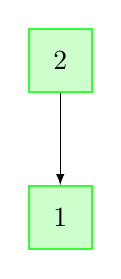
\begin{tikzpicture}
				\node[circle] (b) [commit]{2};
				\node[circle] (a) [commit, below of=b, node distance=2cm]{1};
				\draw[-latex] (b) -- (a);
			\end{tikzpicture}
		\end{column}
	\end{columns}
\end{frame}

\begin{frame}[fragile]
	\frametitle{Beispiele}
	\framesubtitle{Branchen und Mergen}
	\begin{columns}[T]
		\begin{column}{7.5cm}
			\begin{verbatim}
			$ git status
			# On branch master
			\end{verbatim}

			\begin{verbatim}
			$ git checkout -b new-branch
			$ git branch
			\end{verbatim}

			\begin{verbatim}
			$ echo "Lorem ipsum" >> README
			$ git add README
			$ commit -m "Add noise" # (3)
			\end{verbatim}

			\begin{verbatim}
			$ git diff master
			$ git checkout master
			$ git merge new-branch
			$ git branch -d new-branch
			\end{verbatim}
		\end{column}
		\begin{column}{2.5cm}
			\begin{tikzpicture}
				\node[circle] (a) [commit, above right of=b, node distance=2cm]{3};
				\node[circle] (b) [commit]{2};
				\node[circle] (c) [commit, below of=b, node distance=2cm]{1};
				\draw[-latex] (b) -- (c);
				\draw[-latex] (a) -- (b);
			\end{tikzpicture}
		\end{column}
	\end{columns}
\end{frame}

\begin{frame}
	\fontsize{30}{10}\selectfont Äääähm!
	\vspace*{0.5cm}

	\fontsize{20}{10}\selectfont war da nicht was mit \emph{distributed}?!1elf
\end{frame}

\begin{frame}[fragile]
	\frametitle{Beispiele}
	\framesubtitle{Remotes}
	\begin{verbatim}
	$ git clone https://github.com/bup/bup.git
	$ git remote rename origin upstream
	\end{verbatim}

	\begin{verbatim}
	# Änderungen holen
	$ git fetch upstream
	$ git merge upstream/master
	\end{verbatim}

	\begin{verbatim}
	# Änderungen hochladen
	$ git push upstream master
	\end{verbatim}
\end{frame}

\begin{frame}
	\frametitle{Beispiele}
	\framesubtitle{Remotes (Hosting-Optionen)}
	\begin{itemize}
		\item
			GitHub\\
			kostenlos für OpenSource, kostenlose Studenten-Accounts\\
			\url{https://github.com}
		\item
			RBG\\
			kostenlos an der Uni\\
			\url{https://scm.rbg.informatik.tu-darmstadt.de}
		\item
			Gitolite\\
			selber hosten\\
			\url{https://github.com/sitaramc/gitolite}
	\end{itemize}
\end{frame}

\begin{frame}
	\fontsize{30}{10}\selectfont Aber, aber\ldots
	\vspace*{0.5cm}

	\fontsize{20}{10}\selectfont upstream sind Änderungen und ich habe
	Änderungen\ldots\ und\ldots\ und\ldots\ jetzt?
\end{frame}

\begin{frame}[fragile]
	\frametitle{Beispiele}
	\framesubtitle{Rebase}
	\begin{columns}[T]
		\begin{column}{7.5cm}
			\begin{verbatim}
			# Lokale Änderungen auf Basis
			# von upstream/master
			$ echo "..." >> README
			$ git add README
			$ git commit -m "..." # (3)
			\end{verbatim}

			\begin{verbatim}
			# Änderungen holen
			$ git fetch upstream # (4)
			\end{verbatim}
		\end{column}
		\begin{column}{2.5cm}
			\begin{tikzpicture}
				\node[circle] (a1) [commit, above of=b, node distance=2cm]{4};
				\node[circle] (a2) [commit, above right of=b, node distance=2cm]{3};
				\node[circle] (b) [commit]{2};
				\node[circle] (c) [commit, below of=b, node distance=2cm]{1};
				\draw[-latex] (b) -- (c);
				\draw[-latex] (a1) -- (b);
				\draw[-latex] (a2) -- (b);
			\end{tikzpicture}
		\end{column}
	\end{columns}
\end{frame}

\begin{frame}[fragile]
	\frametitle{Beispiele}
	\framesubtitle{Rebase}
	\begin{columns}[T]
		\begin{column}{7.5cm}
			\begin{verbatim}
			# Lokale Änderungen auf Basis
			# von upstream/master
			$ echo "..." >> README
			$ git add README
			$ git commit -m "..." # (3)
			\end{verbatim}

			\begin{verbatim}
			# Änderungen holen
			$ git fetch upstream # (4)
			\end{verbatim}

			\begin{verbatim}
			# Eigene Änderungen auf Upstream
			# anwenden
			$ git rebase upstream/master
			\end{verbatim}
		\end{column}
		\begin{column}{2.5cm}
			\begin{tikzpicture}
				\node[circle] (a1) [commit, above of=b, node distance=2cm]{4};
				\node[circle] (a2) [commit, above right of=a1, node distance=2cm]{3};
				\node[circle] (b) [commit]{2};
				\node[circle] (c) [commit, below of=b, node distance=2cm]{1};
				\draw[-latex] (b) -- (c);
				\draw[-latex] (a1) -- (b);
				\draw[-latex] (a2) -- (a1);
			\end{tikzpicture}
		\end{column}
	\end{columns}
\end{frame}

\begin{frame}
	\fontsize{30}{10}\selectfont zOMG!
	\vspace*{0.5cm}

	\fontsize{20}{10}\selectfont alles kaputt!!!
	\vspace*{0.25cm}

	\only<2> {
		\fontsize{20}{10}\selectfont reflog to the rescue!
	}
\end{frame}

\begin{frame}[fragile]
	\frametitle{reflog}
	\fontsize{6}{10}\selectfont reflog to the rescue!
	\begin{verbatim}
	$ git reflog
	60f023c HEAD@{0}: checkout: moving from git-in-depth to ophase
	6ed550f HEAD@{1}: checkout: moving from ophase to git-in-depth
	60f023c HEAD@{2}: checkout: moving from 60f023cf1991929157518fbb54f2282f77cc6d1b to ophase
	60f023c HEAD@{3}: checkout: moving from git-in-depth to 60f023cf1991929157518fbb54f2282f77cc6d1b
	6ed550f HEAD@{4}: checkout: moving from git-in-depht to git-in-depth
	6ed550f HEAD@{5}: checkout: moving from master to git-in-depht
	6ed550f HEAD@{6}: commit: mrmcd
	60f023c HEAD@{7}: commit: Ophase SS12
	ae6424d HEAD@{8}: commit: Import talk version from Ophase WS11/12
	538f510 HEAD@{9}: commit (initial): init
	\end{verbatim}
\end{frame}

\begin{frame}[fragile]
	\frametitle{Commit Messages}
	\fontsize{8}{8}\selectfont
	\begin{verbatim}
	Capitalized, short (50 chars or less) summary

	More detailed explanatory text, if necessary.  Wrap it to about 72
	characters or so.  In some contexts, the first line is treated as the
	subject of an email and the rest of the text as the body.  The blank
	line separating the summary from the body is critical (unless you omit
	the body entirely); tools like rebase can get confused if you run the
	two together.

	Write your commit message in the present tense: "Fix bug" and not "Fixed
	bug."  This convention matches up with commit messages generated by
	commands like git merge and git revert.

	Further paragraphs come after blank lines.

	- Bullet points are okay, too

	- Typically a hyphen or asterisk is used for the bullet, preceded by a
	  single space, with blank lines in between, but conventions vary here

	- Use a hanging indent
	\end{verbatim}
	\url{http://tbaggery.com/2008/04/19/a-note-about-git-commit-messages.html}
\end{frame}

\begin{frame}
	\frametitle{Cooler Scheiß\texttrademark}
	\begin{itemize}
		\item
			interactive Rebase
		\item
			Index
		\item
			Hooks
		\item
			Sicher gegen Manipulation
		\item
			bup
	\end{itemize}
\end{frame}

\section{Tools}
\begin{frame}
	\fontsize{30}{10}\selectfont Tools
\end{frame}

\begin{frame}
	\frametitle{Tools}
	\begin{itemize}
		\item
			tig
		\item
			gitk
		\item
			gitg
		\item
			Tower Git
		\item
			gitkx
	\end{itemize}
\end{frame}

\begin{frame}
	\frametitle{Weiterführendes / Nachschlagewerk}
	\begin{itemize}
		\item
			\url{http://progit.org/}
		\item
			\url{http://gitref.org/}
		\item
			\url{http://sea.ucar.edu/event/unlocking-secrets-git}
		\item
			\url{http://blip.tv/scott-chacon}
		\item
			28c3: bup: Git for backups\\
			\url{http://www.youtube.com/watch?v=u_rOi2OVvwU}
	\end{itemize}
\end{frame}

\begin{frame}[fragile]
	\frametitle{Danke}
	\begin{itemize}
		\item
			\verb|zorzar| auf freenode \& hackint
		\item
			zz@zoranzaric.de (Email \& Jabber)
		\item
			\url{zoranzaric.de}
		\item
			\url{github.com/zoranzaric}
		\item
			\url{gplus.zoranzaric.de}
		\item
			@zoranzaric\\[0.5cm]
		\item
			Slides: \url{zoranzaric.de/git-ophase1213.pdf}
	\end{itemize}
\end{frame}

\begin{frame}
	\includegraphics{qr-code.png}
\end{frame}

\end{document}
